\section{Task 4 --- Index Selection and Evaluation}

All final index timings use the largest database (987{,}686 sales) and the unchanged Task~3 queries.
For each query and condition, we perform one untimed warm-up followed by five timed runs, measuring client time around \texttt{execute} and \texttt{fetchall}. We report the mean and sample standard deviation. Percentage changes use the means rounded to two decimal places, following \texttt{task4\_summary.csv}.
The project's ``noticeable'' rule requires both a plan change and an absolute mean change larger than 10\% of the un-indexed mean \emph{and} larger than two un-indexed sample standard deviations.
We use this as a descriptive threshold for interpreting the measurements.

\subsection{What the plans suggest}
Without extra indexes, only Q1 and Q6 filter \texttt{resale\_transaction} on \texttt{transaction\_month}, keeping 80{,}306 of 987{,}686 rows (8.1\%) and discarding the rest (saved plans under \path{Task 4/results/plans/}).
Q2--Q5 read essentially every sale, so an index has little to skip.
An earlier four-index experiment was reported to slow Q1 and led us to test candidates separately. Its original spreadsheet is unavailable, so we retain it only as context for the experimental design.

\subsection{Candidate screening (summary)}
Nine candidates were created one at a time, analysed, timed on Q1--Q6, and dropped
(\path{task4_candidate_screening.csv}, 330 rows).
Percentages compare each candidate to a \emph{pooled} un-indexed baseline of ten runs (before the first and after the last candidate).
Those two baseline blocks disagree---especially Q1 (26.30 vs 21.06~ms) and Q6 (32.89 vs 40.32~ms), the latter including slow end runs of 50.3 and 47.8~ms---so pooled percentages must be read with that drift in mind.
The slow ending baseline inflates the pooled mean, so negative Q6 percentages require caution.

Table~\ref{tab:screen} summarises the screening results.
Only month-based indexes clearly helped Q1 under the noticeability rule.
\texttt{flat\_id} indexes made Q6 much slower when the planner used them.
The remaining indexes on flat type, town and proximity columns had no noticeable effect under the rule.
Figure~\ref{fig:heat} shows the heat map drawn from the same pooled percentages.

\begin{table}[H]
\centering
\caption{Candidate screening on step~5 (pooled baseline). Build time is CREATE only. Source: \texttt{task4\_candidate\_summary.csv}.}
\label{tab:screen}
\footnotesize
\begin{tabular}{@{}clrrll@{}}
\toprule
ID & Index (abbrev.) & Size (MB) & Build (ms) & Q1 vs pool & Verdict \\
\midrule
C1 & B-tree(\texttt{transaction\_month}) & 6.73 & 130.1 & $-35.8\%$ & \textbf{kept} \\
C2 & covering month & 29.73 & 409.4 & $-39.3\%$ & reject (size) \\
C3 & BRIN(\texttt{transaction\_month}) & 0.02 & 23.8 & $-31.8\%$ & not submitted \\
C4 & B-tree(\texttt{flat\_id}) & 9.72 & 202.0 & noise & reject (Q6 $+66.6\%$) \\
C5 & covering \texttt{flat\_id} & 29.73 & 495.0 & noise & reject \\
C6--C9 & type / town / hawker / prox.\ covering & $\le 0.99$ & $\le 29.8$ & noise & reject \\
\bottomrule
\end{tabular}
\end{table}

\begin{figure}[H]
\centering
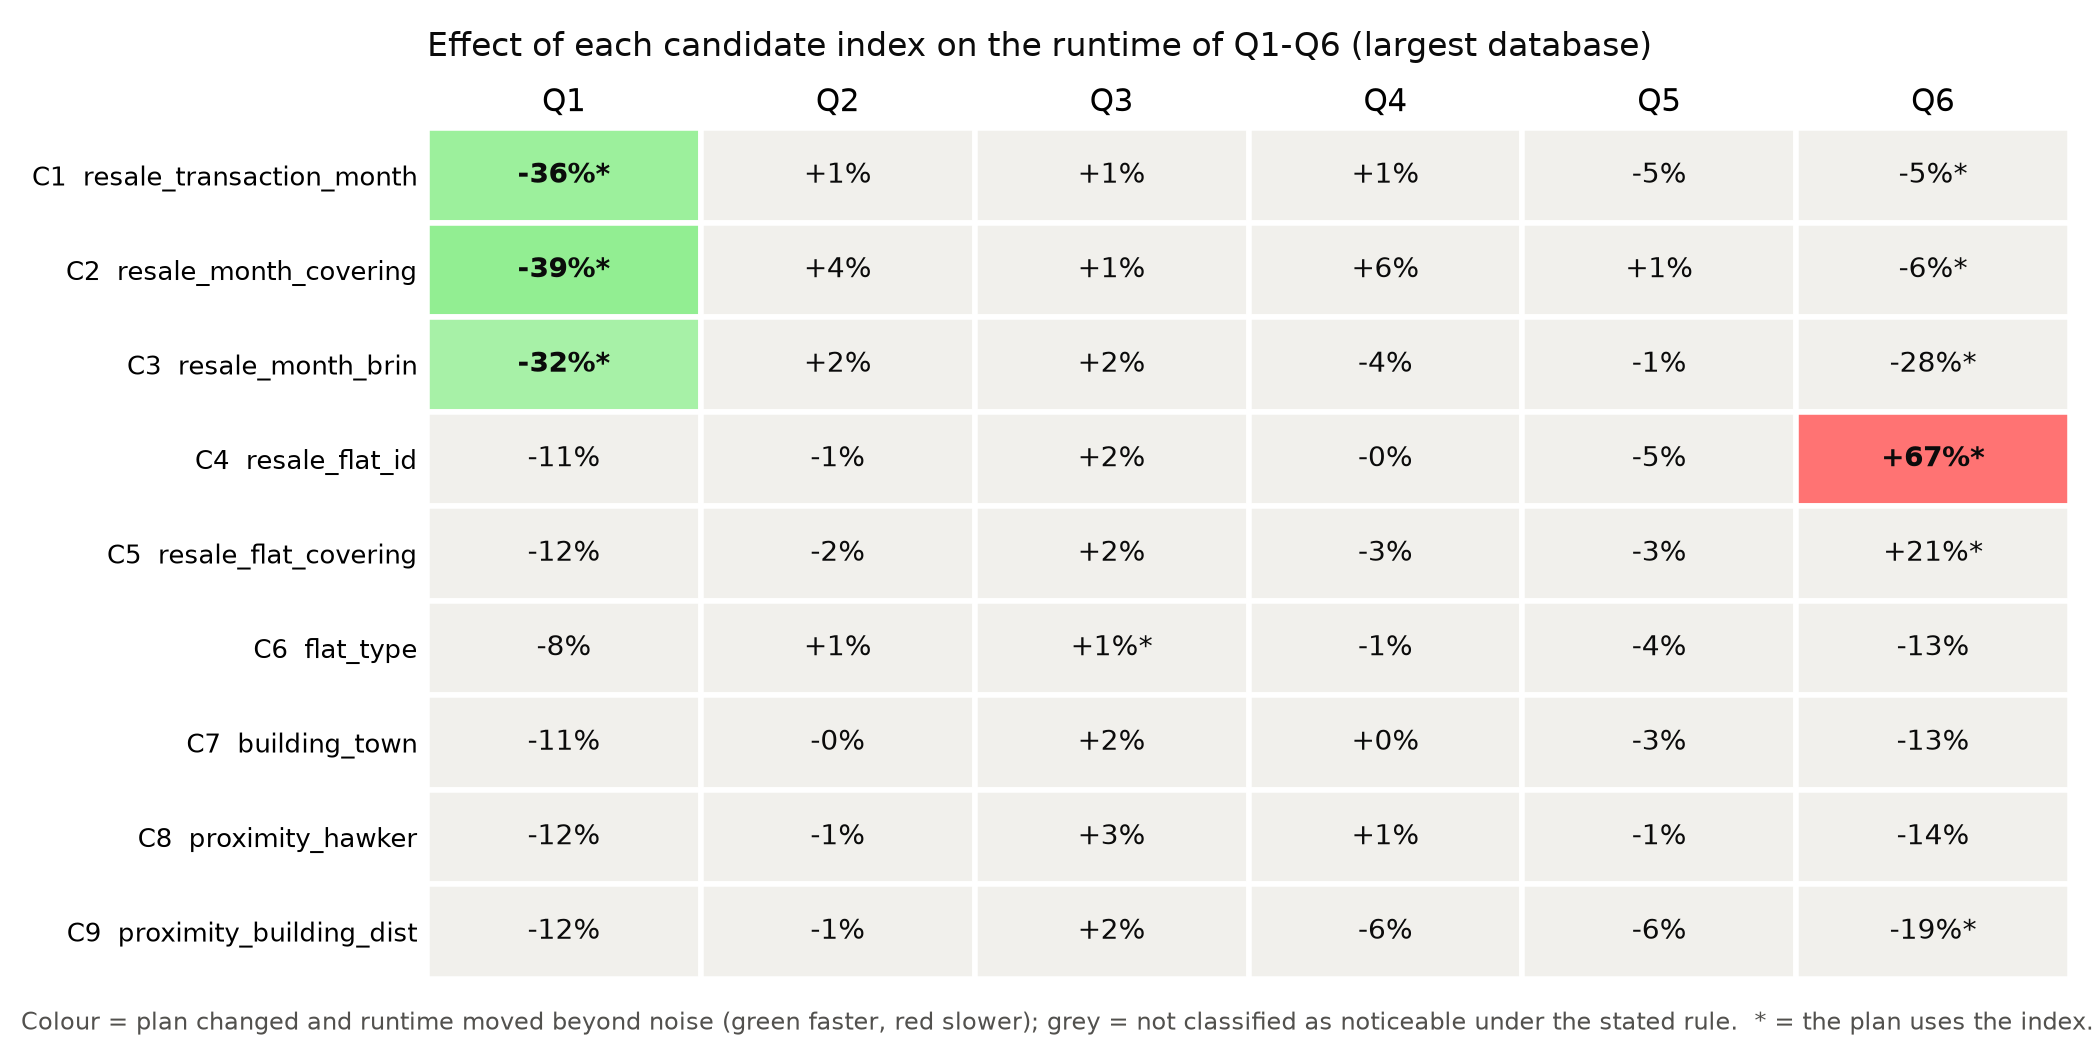
\includegraphics[width=0.95\textwidth]{figures/task4_candidate_screening.png}
\caption{Screening heat map: percent change versus pooled baseline. Asterisk marks index use in the plan. Grey cells fail the project's noticeability rule.}
\label{fig:heat}
\end{figure}

Combinations of C1 with other candidates did not improve Q1 beyond the mid-teens of milliseconds in a way that justified extra indexes (\texttt{task4\_combination\_tests.csv}).
The submitted index is judged from the same-session with/without experiment below, not from screening percentages alone.

\subsection{Final index}
We submit a plain B-tree on the date column (full file in Appendix~\ref{app:indexes}):
\begin{verbatim}
CREATE INDEX idx_resale_transaction_month
    ON housing.resale_transaction (transaction_month);
ANALYZE housing.resale_transaction;
\end{verbatim}
The B-tree targets the selective date filter. Its usefulness is less dependent on physical row ordering than the BRIN alternative.
In screening, the covering B-tree reduced Q1 runtime by a further $0.85\,\mathrm{ms}$ but occupied $4.4\times$ as much space.
BRIN recorded a lower Q6 mean against the drifted baseline, but we chose the B-tree to avoid relying on the ordering produced by the CSV load.

\subsection{Final with/without measurement}
Table~\ref{tab:final} and Figure~\ref{fig:t4bars} show the final comparison from Part~C of the notebook.
Each query was measured five times before and after applying \texttt{indexes.sql}, giving 60 records.
Both conditions contain 987{,}686 transactions. Total database size is 124.01~MB without the index and 130.75~MB with it, compared with 104.87~MB in Task~3 at step~5.
These values use the same database-size function but were recorded at different stages. The files do not establish the cause of the Task~3/4 size difference, so the Task~3 line is a historical reference. We assess the index using the matched Task~4 conditions.

\begin{table}[H]
\centering
\caption{Final index effect on step~5 (mean $\pm$ sample SD, ms). Source: \texttt{task4\_summary.csv}.}
\label{tab:final}
\footnotesize
\begin{tabular}{@{}lrrrl@{}}
\toprule
Query & Without index & With index & Change & Index used \\
\midrule
Q1 & $21.56 \pm 0.25$ & $14.93 \pm 0.32$ & $-30.8\%$ ($1.44\times$) & yes \\
Q2 & $392.17 \pm 3.93$ & $386.40 \pm 5.59$ & $-1.5\%$ (plan unchanged) & no \\
Q3 & $212.18 \pm 0.48$ & $208.10 \pm 0.89$ & $-1.9\%$ (plan unchanged) & no \\
Q4 & $69.97 \pm 0.80$ & $70.32 \pm 0.49$ & $+0.5\%$ (plan unchanged) & no \\
Q5 & $209.47 \pm 6.36$ & $205.62 \pm 2.69$ & $-1.8\%$ (plan unchanged) & no \\
Q6 & $32.62 \pm 1.64$ & $34.61 \pm 0.15$ & $+6.1\%$ & yes \\
\bottomrule
\end{tabular}
\end{table}

\begin{figure}[H]
\centering
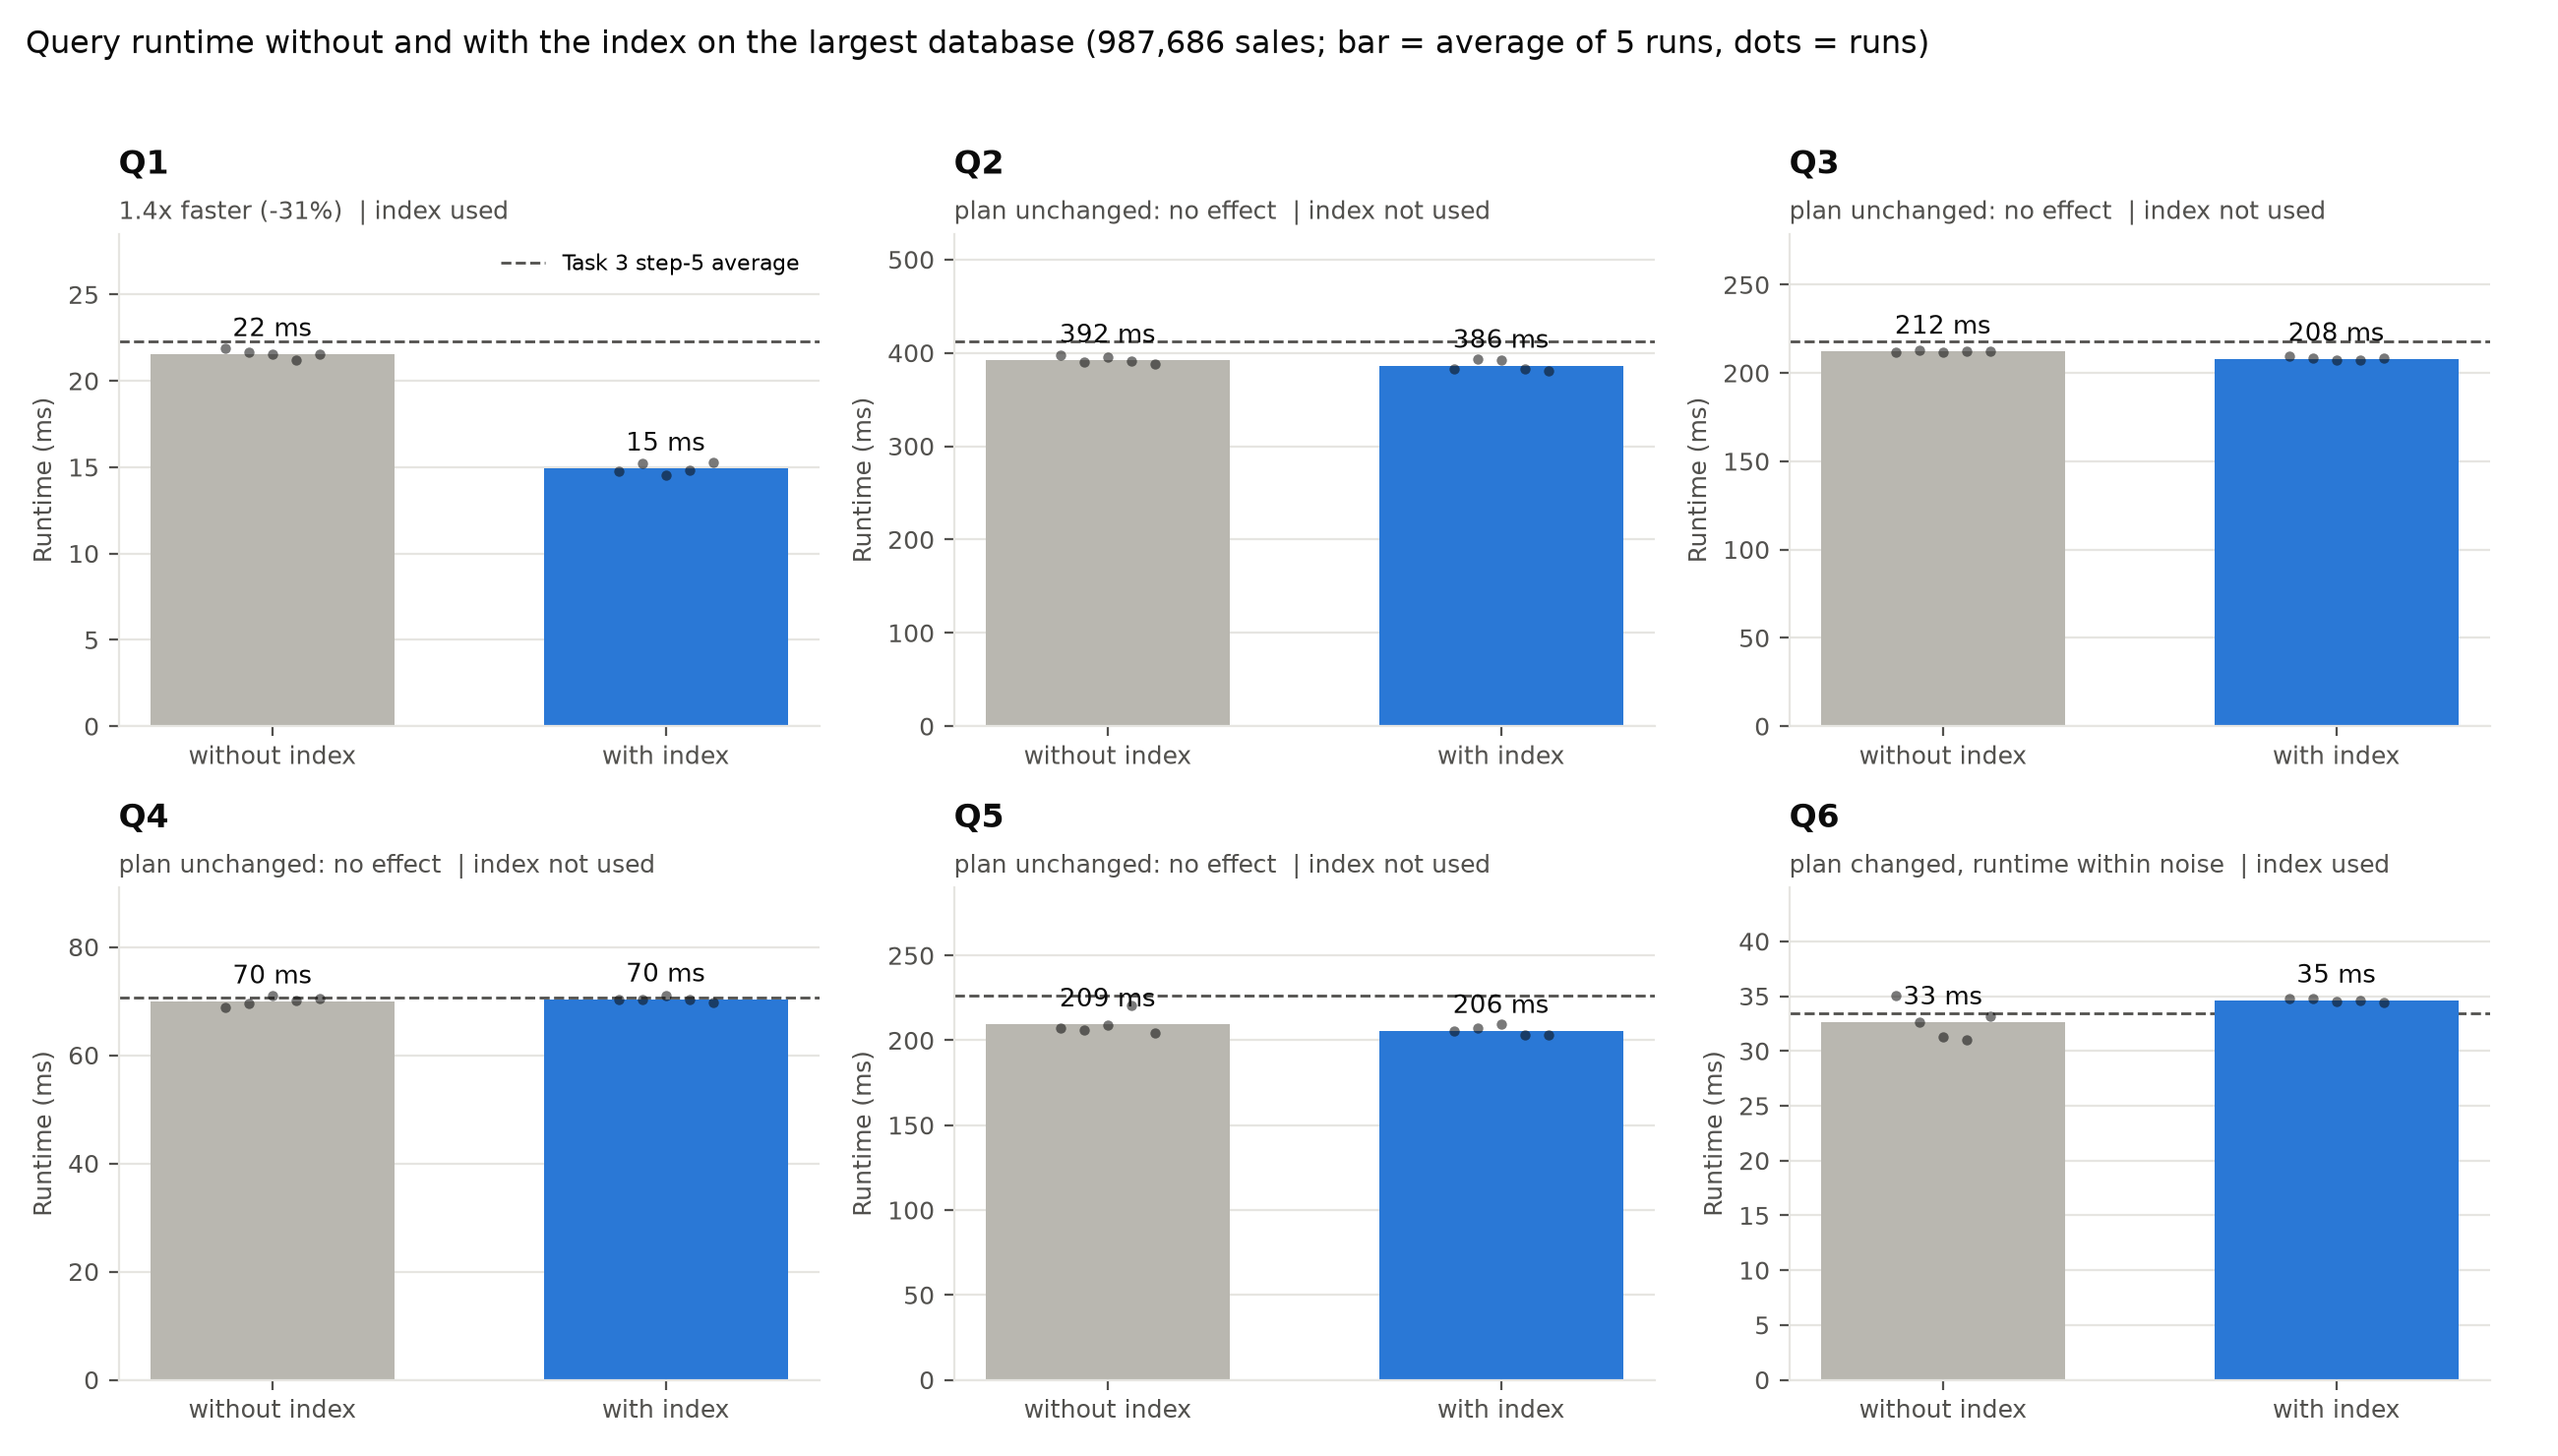
\includegraphics[width=\textwidth]{figures/task4_runtime_with_vs_without_index.png}
\caption{Average client runtime without and with the submitted index (five runs; dots are individual timed runs). Dashed line: Task~3 step~5 average.}
\label{fig:t4bars}
\end{figure}

\paragraph{Q1.}
The plan changes from a parallel sequential scan with a date filter to a parallel bitmap heap scan fed by a bitmap index scan on \texttt{idx\_resale\_transaction\_month}, returning the 80{,}306 matching rows.
Client mean runtime falls by $6.63\,\mathrm{ms}$ ($-30.8\%$).
The saved \texttt{EXPLAIN ANALYZE} plans support this change in access method. Their instrumented server execution times are separate from the client averages reported here.

\paragraph{Q6.}
The planner uses the index and the client mean rises by about $1.99\,\mathrm{ms}$ ($+6.1\%$).
The change is below both runtime thresholds, approximately $3.26\,\mathrm{ms}$ and $3.28\,\mathrm{ms}$.
The five with-index runs ($34.41$--$34.76\,\mathrm{ms}$) overlap the without-index range ($31.02$--$35.09\,\mathrm{ms}$).
We report the measured increase without calling it a noticeable regression under the project rule.

\paragraph{Q2--Q5.}
Plans are identical with and without the index; differences between $-1.9\%$ and $+0.5\%$ are treated as noise.

\subsection{Cost of the index}
The index occupies $6.73\,\mathrm{MB}$, or $13.7\%$ of the $49.1\,\mathrm{MB}$ table heap. Executing \texttt{indexes.sql}, including \texttt{ANALYZE}, took $148.4\,\mathrm{ms}$. These measurements are saved in \texttt{task4\_index\_cost.csv}.
Inserting 100{,}000 existing sales into a scratch copy averaged $203.0\,\mathrm{ms}$ without the index and $288.9\,\mathrm{ms}$ with it ($+42.4\%$, three runs per condition). The notebook prints rounded single-run times of 206/227/176~ms and 300/283/283~ms. The reported means use the underlying unrounded measurements.
The analytical workload is read-mostly after load, so the insert penalty is acceptable here.

\subsection{Other performance experiments}
Raising session \texttt{work\_mem} to 256~MB removed Q2's sort spill (saved plan shows about $14{,}824\,\mathrm{kB}$ disk under default settings) and moved the five-run mean from $417.0\,\mathrm{ms}$ (inflated by one $532\,\mathrm{ms}$ run) to $356.4\,\mathrm{ms}$.
Declaring Q3's \texttt{WITH three\_room} as \texttt{NOT MATERIALIZED} cut the mean from $210.2\,\mathrm{ms}$ to $109.9\,\mathrm{ms}$ ($-47.7\%$) with identical results. This improvement came from a SQL rewrite.
We did not change \texttt{queries.sql}.
